\chapter{Cuestionario}
\begin{enumerate}
	\item Leer la documentación “rpn tutorial” de rrdtool
	\item Leer la documentación “cdef tutorial” de rrdtool
	\begin{itemize}
		\item ¿Qué son las CDEFs?
		\item ¿Qué son las expresiones RPN?
	\end{itemize}
	\item Leer la documentación  “rrdgraph\_rpn” de rrdtool
	\begin{itemize}
		\item ¿Qué diferencia hay entre CDEF y VDEF?
		\item ¿Para qué sirve el operador COUNT?
		\item ¿Para qué sirve el operador POP?
		\item ¿Para qué sirve LSLSLOPE?
		\item ¿Para qué sirve LSLINT?
	\end{itemize}
	\item Ejercicio 1 – Sello 1 – Resolver el cuestionario
	\item Ejercicio 2 – Sello 2 - Resolver los siguientes ejercicios a mano.
	\begin{itemize}
		\item CDEF:bits=inoctets,8,* (inoctets = [1,2,3,4])
		\item CDEF:avg=in,out,+,2,/ (in = [1,2,3,4], out = [5,6,7,8])
		\item CDEF:bigger=x,y,MAX (x = [1,2,3,4], y = [5,6,7,8])
		\item CDEF:bigger=x,y,GT,x,y,IF (x = [1,8,3,10], y = [5,6,7,8])
		\item CDEF:unzero=x,UN,0,x,IF (x = [UN,8,UN,10])
		\item CDEF:avg2=v1,v2,v3,3,AVG (v1 = [1,8,3,10], v2 = [5,6,7,8], v3= [1,2,3,4])
	\end{itemize}
	\item Ejercicio 3 – Sello 3 -  Usar SNMP para monitorizar dos valores. Usar rrdtool para crear dos colecciones (DS) almacenar la información usando SNMP. Usar operadores booleanos, aritméticos y comparacíon de  valores para graficar la información recopilada.
\end{enumerate}
\noindent
En las siguientes fotos, se pueden apreciar las repuestas y el desarrollo de cada una de las preguntas y ejercicios anteriores.
\begin{figure}[H]
	\centering
	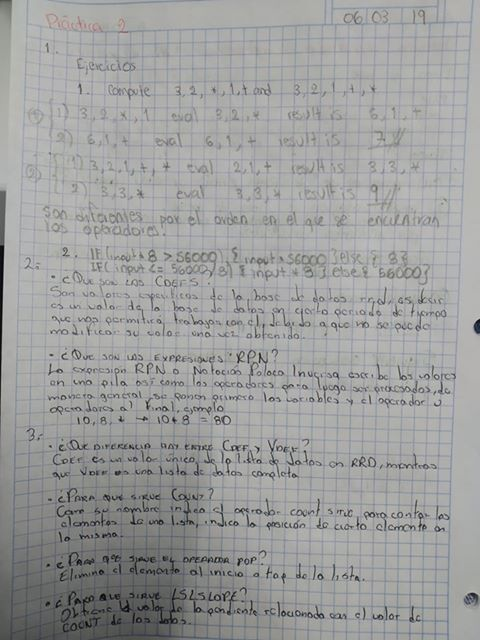
\includegraphics[scale=.85]{imagenes/practica/p2-1.jpg}
\end{figure}
\begin{figure}[H]
	\centering
	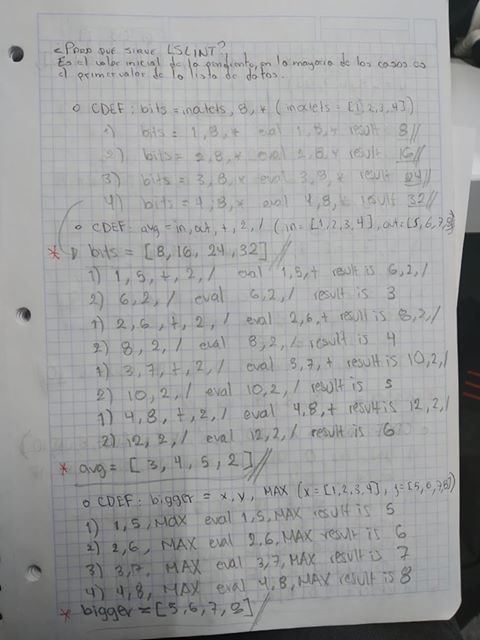
\includegraphics[scale=1]{imagenes/practica/p2-2.jpg}
\end{figure}
\begin{figure}[H]
	\centering
	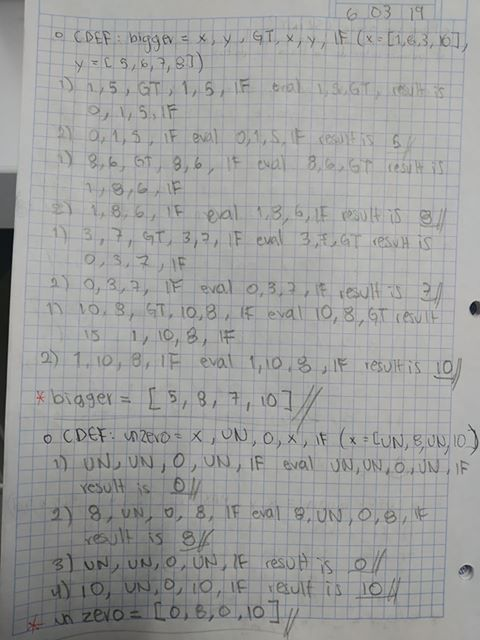
\includegraphics[scale=1]{imagenes/practica/p2-3.jpg}
\end{figure}
\begin{figure}[H]
	\centering
	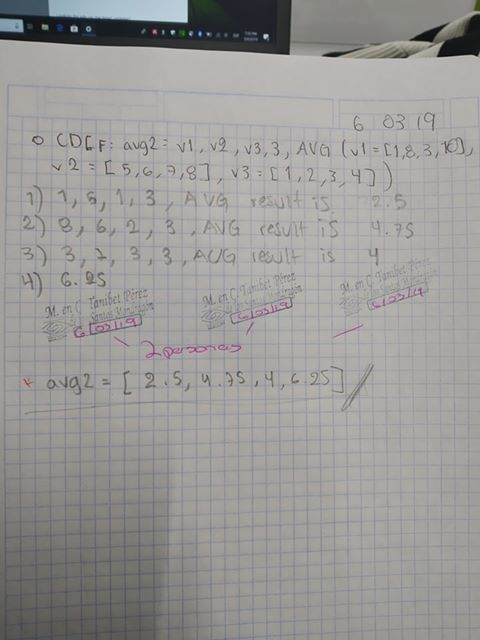
\includegraphics[scale=1]{imagenes/practica/p2-4.jpg}
\end{figure}